\documentclass[a4paper]{article}

%%%%%%%% CREATE DOCUMENT STRUCTURE %%%%%%%%
%% Language and font encodings
\usepackage[spanish]{babel}
\usepackage[utf8x]{inputenc}
\usepackage[T1]{fontenc}
%\usepackage{subfig}

\usepackage{listings} % Para incluir código
\usepackage{xcolor}   % Colores para el código

% Configuración de estilo
\lstset{
    basicstyle=\ttfamily\small, % Fuente monoespaciada
    numbers=left,               % Números de línea a la izquierda
    numberstyle=\tiny\color{gray},
    keywordstyle=\color{blue},
    commentstyle=\color{green!50!black},
    stringstyle=\color{red!70!black},
    breaklines=true,            % Saltar líneas largas
    frame=single,               % Marco alrededor del código
    tabsize=4
}

%% Sets page size and margins
\usepackage[a4paper,top=3cm,bottom=2cm,left=2cm,right=2cm,marginparwidth=1.75cm]{geometry}

%% Useful packages
\usepackage{amsmath}
\usepackage{graphicx}
\usepackage[colorinlistoftodos]{todonotes}
%\usepackage[colorlinks=true, allcolors=blue]{hyperref}
\usepackage{caption}
\usepackage{subcaption}
\usepackage{sectsty}

\usepackage{float}
\usepackage{titling} 

%% Referencias/Bibliografía
%\usepackage[backend=biber, style=apa]{biblatex}
%\addbibresource{ref.bib} % Nombre del archivo con las referencias


\usepackage[colorinlistoftodos]{todonotes}
\usepackage{xcolor}
\definecolor{darkgreen}{rgb}{0.0, 0.4, 0.0}


%Links de referencias
\usepackage[hidelinks]{hyperref} % Hace que las referencias sean clicables
\newcommand{\myref}[1]{\textsuperscript{\textbf{\ref{#1}}}} % Define un estilo propio

%%%%%%%% DOCUMENT %%%%%%%%
\begin{document}

%%%% Title Page
\begin{titlepage}

\newcommand{\HRule}{\rule{\linewidth}{0.5mm}} 							% horizontal line and its thickness
\center 
 
% University
\textsc{\LARGE Universidad de Granada}\\[1cm]

% Document info
\textsc{\Large Periféricos y Dispositivos de Interfaz Humana}\\[0.2cm]
\textsc{\large Curso 2025/2026}\\[1cm] 										% Course Code
\HRule \\[0.8cm]
{ \huge \bfseries Proyecto. Código Morse usando Arduino}\\[0.7cm]								% Assignment
\HRule \\[2cm]
\large
\emph{Autora:}\\
Inés Ruiz Sánchez\\[1.5cm]													% Author info
{\large \today}\\[5cm]
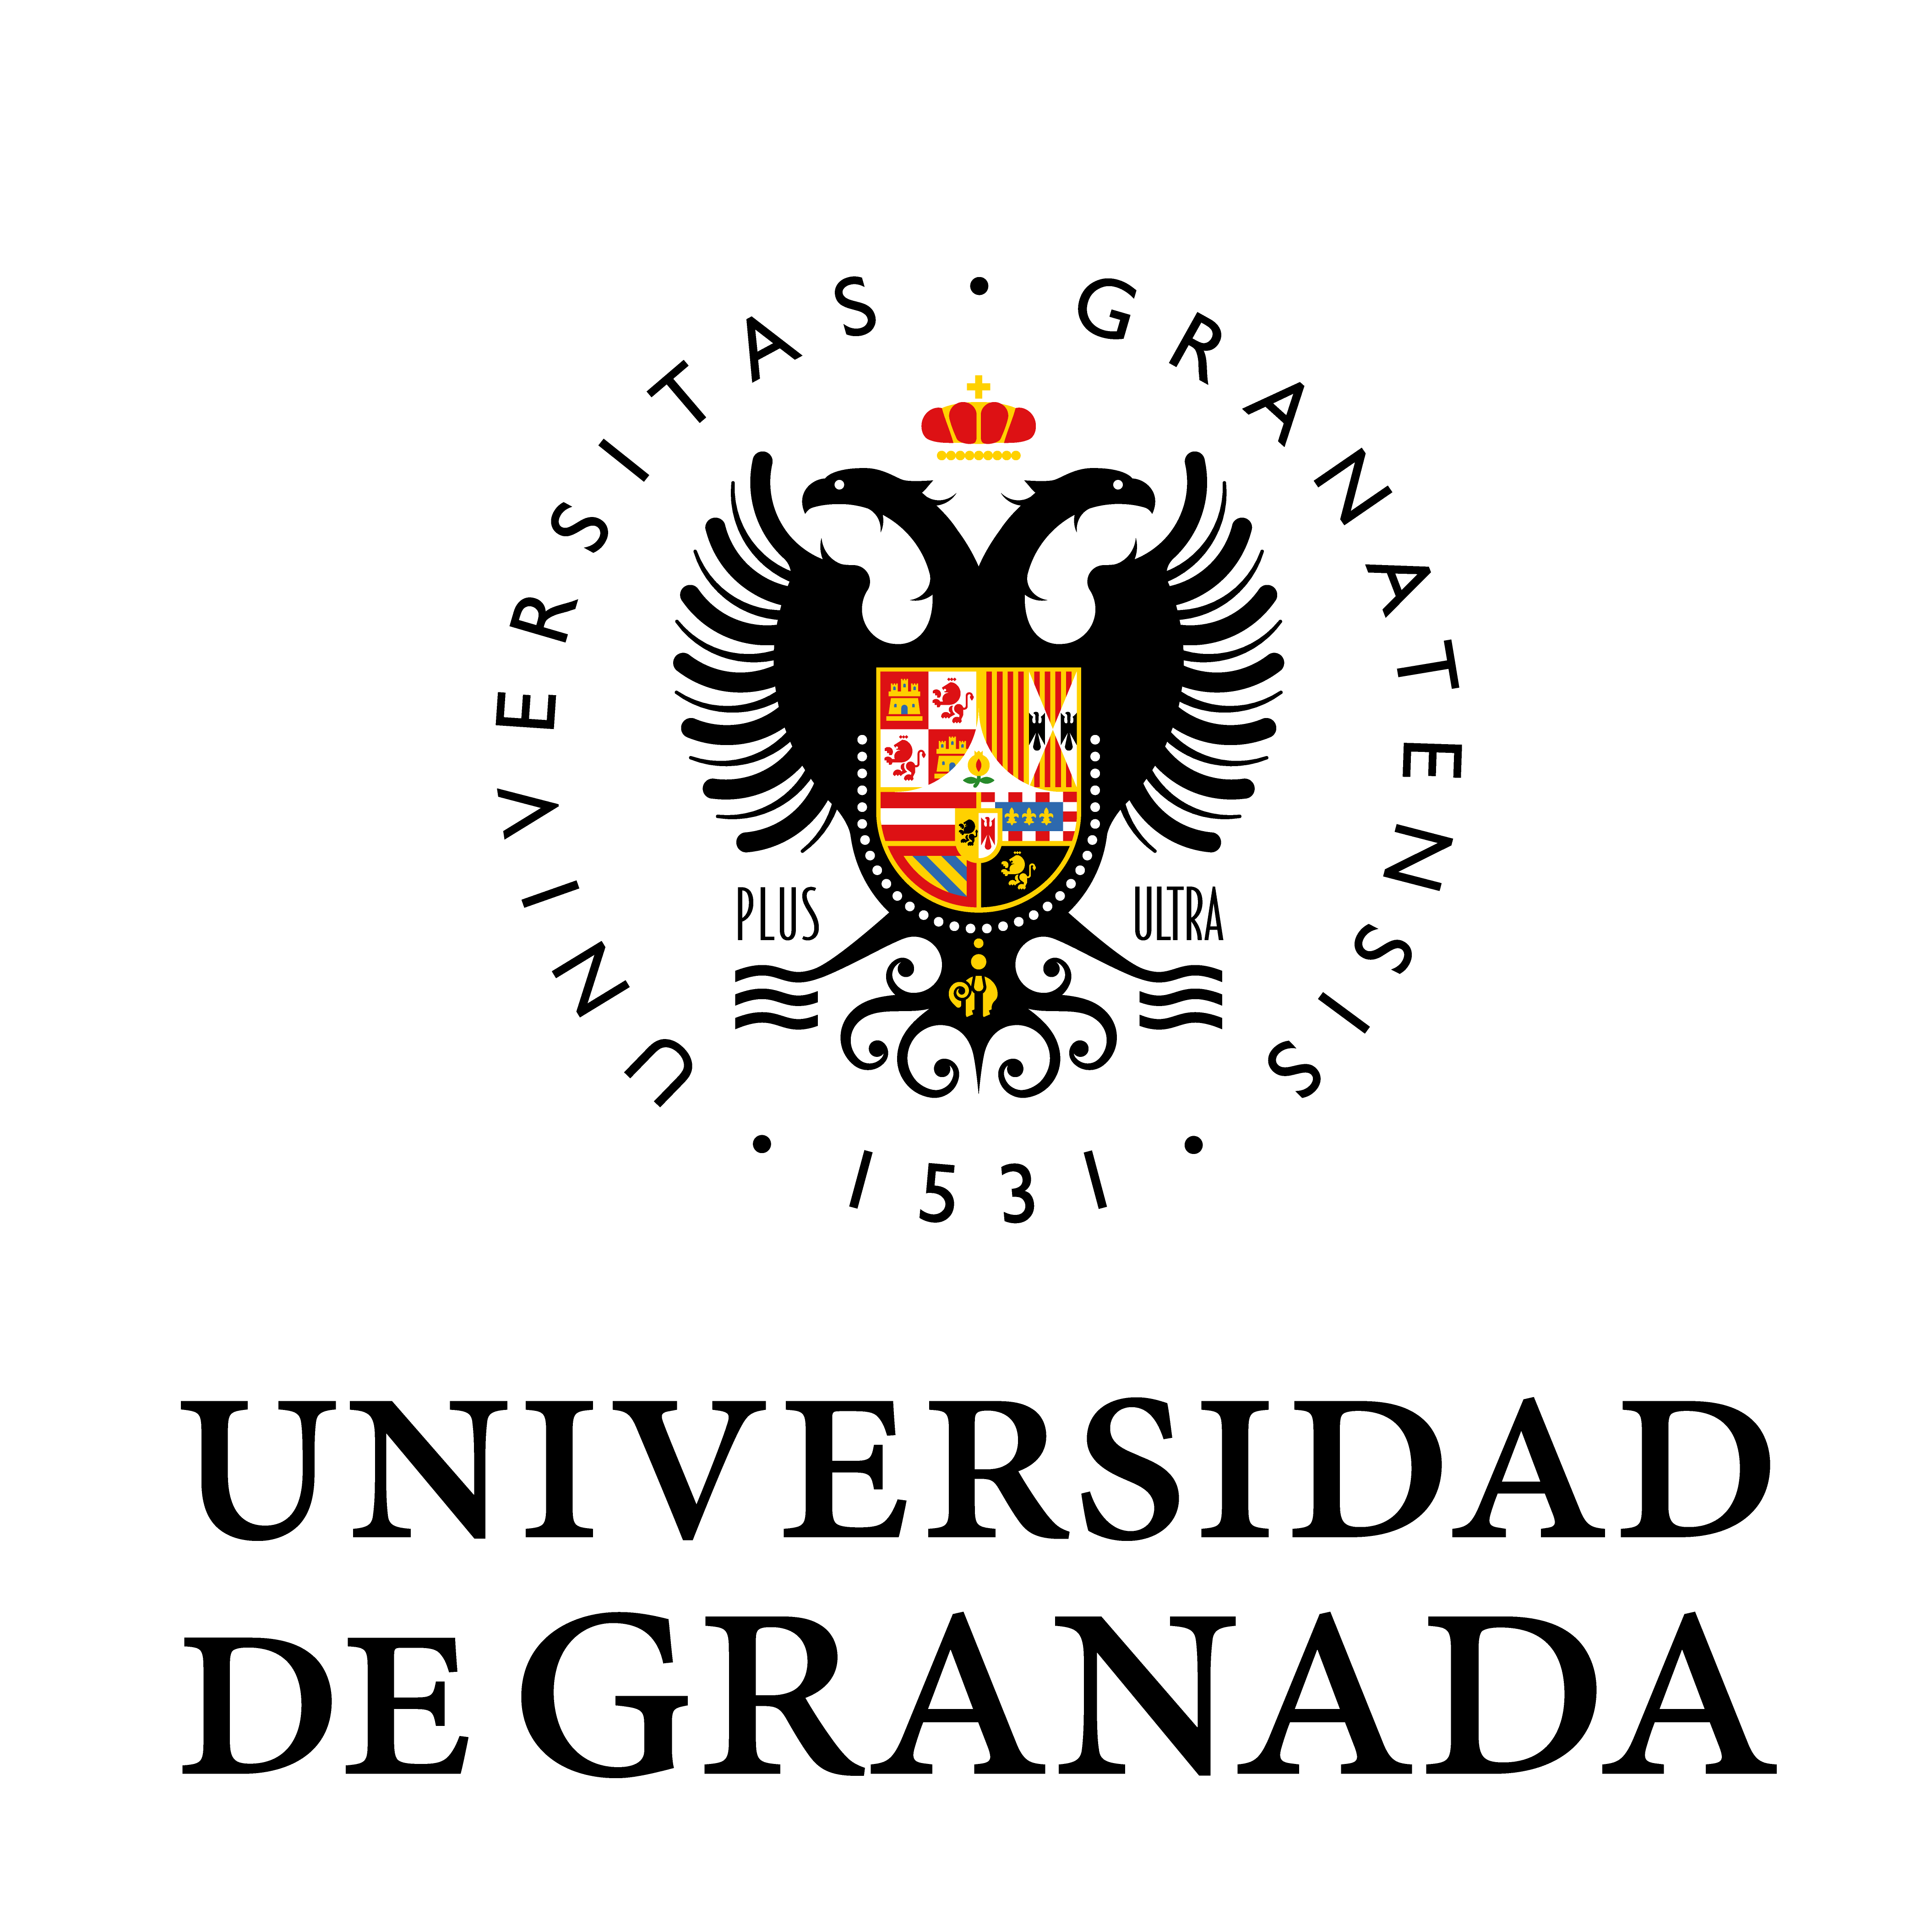
\includegraphics[width=0.3\textwidth]{images/UGRlogo.png}\\[1cm] 	% University logo
\vfill 
\end{titlepage}

%%\begin{abstract}
%%Your abstract.
%%\end{abstract}

% Generar índice de contenidos y figuras
\tableofcontents
%\newpage
\listoffigures
\newpage

%%%% SECTIONS
\section{Introducción}\label{sec:1_intro}
% SECCIÓN 1. INTRODUCCIÓN
\subsection{¿Qué es el código Morse y por qué es interesante?}
\begin{itemize}
    \item La duración de una raya es tres veces la de un punto
    \item El tiempo que transcurre entre cada raya o punto es igual a la duración de un punto
    \item El espacio entre dos letras tiene la misma longitud que la raya
    \item El espacio entre dos palabras tiene la misma duración que siete puntos
\end{itemize}
\begin{table}[h]
    \centering
    \renewcommand{\arraystretch}{1.2} % Da un poco más de espacio entre las filas
    \begin{tabular}{|c|c|c|c|c|c|}
    \hline
    \textbf{Letra} & \textbf{Código} & \textbf{Letra} & \textbf{Código} & \textbf{Número} & \textbf{Código} \\ \hline
    A & \textbf{$.-$}    & N & \textbf{$-.$}    & 1 & \textbf{$.----$} \\ \hline
    B & \textbf{$-...$}  & O & \textbf{$---$}   & 2 & \textbf{$..---$} \\ \hline
    C & \textbf{$-.-.$}  & P & \textbf{$.--.$}  & 3 & \textbf{$...--$} \\ \hline
    D & \textbf{$-..$}   & Q & \textbf{$--.-$}  & 4 & \textbf{$....-$} \\ \hline
    E & \textbf{$.$}     & R & \textbf{$.-.$}   & 5 & \textbf{$.....$} \\ \hline
    F & \textbf{$..-.$}  & S & \textbf{$...$}   & 6 & \textbf{$-....$} \\ \hline
    G & \textbf{$--.$}   & T & \textbf{$-$}     & 7 & \textbf{$--...$} \\ \hline
    H & \textbf{$....$}  & U & \textbf{$..-$}   & 8 & \textbf{$---..$} \\ \hline
    I & \textbf{$..$}    & V & \textbf{$...-$}  & 9 & \textbf{$----.$} \\ \hline
    J & \textbf{$.---$}  & W & \textbf{$.--$}   & 0 & \textbf{$-----$} \\ \hline
    K & \textbf{$-.-$}   & X & \textbf{$-..-$}  & \multicolumn{2}{c|}{} \\ \cline{1-4}
    L & \textbf{$.-..$}  & Y & \textbf{$-.--$}  & \multicolumn{2}{c|}{} \\ \cline{1-4}
    M & \textbf{$--$}    & Z & \textbf{$--..$}  & \multicolumn{2}{c|}{} \\ \hline
    \end{tabular}
    \caption{Alfabeto internacional y números en Código Morse}
    \label{tab:morse_alfabeto}
\end{table}

\subsection{Objetivo del proyecto}
\begin{itemize}
    \item \textbf{Codificador} - Modo transmisor. Programar el Arduino para que, dada una cadena de texto (por ejemplo, una palabra escrita en el código o enviada desde el PC por el puerto serie), el Arduino la traduzca y la emita haciendo parpadear un LED y sonando un zumbador (buzzer) con los tiempos exactos del código Morse (punto corto, raya larga).
    \item \textbf{Decodificador} - Modo Receptor. Conectar un pulsador (botón) al Arduino. El usuario hará pulsaciones cortas y largas. El programa deberá medir el tiempo que el botón está pulsado para distinguir entre "puntos" y "rayas", agruparlos, y mostrar por el monitor serie (o en una pequeña pantalla LCD) la letra o palabra que se está tecleando.
\end{itemize}

%----------------------------------------------------------------
\section{Hardware utilizado}\label{sec:2_hw}
\input{secciones/02_hardware}

%----------------------------------------------------------------
\section{Desarrollo del Software (Código)}\label{sec:3_sw}
%----------------------------------------------------------------
\section{Problemas encontrados y soluciones}
%----------------------------------------------------------------
\section{Conclusiones y Posibles Mejoras}


Anexo \ref{anexo:an1}


%----------------------------------------------------------------
%----------------------------------------------------------------

\section{Anexo}

Nota: Las tildes en los trozos de código no se reconocen en LATEX por lo que el carácter no se escribe. Es por eso por lo que o bien no aparece un caracter o bien el caracter no tiene tilde, pareciendo una falta ortográfica.\\
\subsection{Anexo 1} \label{anexo:an1} 
%\lstinputlisting[language=C]{src/ejer1.c}
\href{https://www.tinkercad.com/things/cJ7XJBloj7o/editel?returnTo=%2Fdashboard%2Fcollections%2F45N1xWNxGAp%2Fall&sharecode=4sl_ZT-0OL1J4BYZHna3SUFVUEHoGAx84j9y6vthwKQ}{Circuito en Tinkercad}

\subsection{Anexo 2} \label{anexo:an2} 
%\lstinputlisting[language=C]{src/ejer2.c}

\newpage
%Bibliografía
\begin{thebibliography}{9}
    \bibitem{schernich} 
    E. Schernich y P. Martínez. 
    \textit{Arduino para principiantes: aprendizaje mediante programación por bloques para docentes y toda la familia}. 
    2a ed. Barcelona: Marcombo, 2019.
    
    \bibitem{monk} 
    S. Monk y J. Pompa. 
    \textit{30 proyectos con Arduino}. 
    Madrid: Estribor, 2012.
\end{thebibliography}
\end{document}